
\chapter{Introduction}

\section{Objectives of this Thesis}
Subject of this thesis is the ophthalmic surgical robot developed in the iRAM!S project \cite{iramis}. When performing minimally invasive surgery, an important task is to prevent lateral movement of the tool at the point of incision to minimize strain on the surrounding tissue. In the iRAM!S project, this is achieved by defining a point on the needle as a Remote Center of Motion (RCM) and algorithmically forcing its velocity to zero. This thesis focuses on the following topics regarding the implementation of a virtual RCM:
\begin{itemize}
	\item Recalculation and verification of the Jacobian matrix for the surgical robot, both for unconstrained and constrained movement. For this purpose a model of the robot is implemented in the V-REP simulation environment.
	\item In the simulation environment, performing an injection at multiple sites of the inner eye surface and measuring the deviation of the RCM point  from its optimal position.
	\item Finding a set of control parameters that ensures that the needle pose quickly converges to any target pose within the workspace of the robot while maintaining the RCM position. 
	\item Comparing the performance of the Jacobian pseudoinverse method to V-REPs built-in inverse kinematics solver, which employs a Dampened Least Squares method, to get an estimate for the possible accuracy.
\end{itemize} 

\section{Robotic Assisted Minimally Invasive Surgery}

In recent years, robotic assistance has gained increasing acceptance in clinical practice, mainly due to improvements in precision, reliability and ergonomics. Most of these systems, referred to as \textit{surgical assistants}, are designed to enhance the ability of a surgeon to perform a certain procedure with additional tools. \textit{Surgeon extenders} are operated directly by the surgeon and offer improved instrument control and manoeuvrability by reducing hand tremor or offering more dexterous tool handling inside the patients body. The goal of these devices is to provide treatments for diseases that would be otherwise difficult to handle, decrease error rates and reduce the length of clinical procedures. Besides surgeon extenders, there are auxiliary surgical supports which operate along the surgeon and perform additional tasks such as controlling an endoscope. The surgeon can either steer the tool through an interface or the surcigal support may be autonomous to some degree. One of the most well-known robotic assistance devices currently used in clinical practice is the Da Vinci Surgical System \cite{DaVinci}.

\begin{figure}[t!]
	\centering
	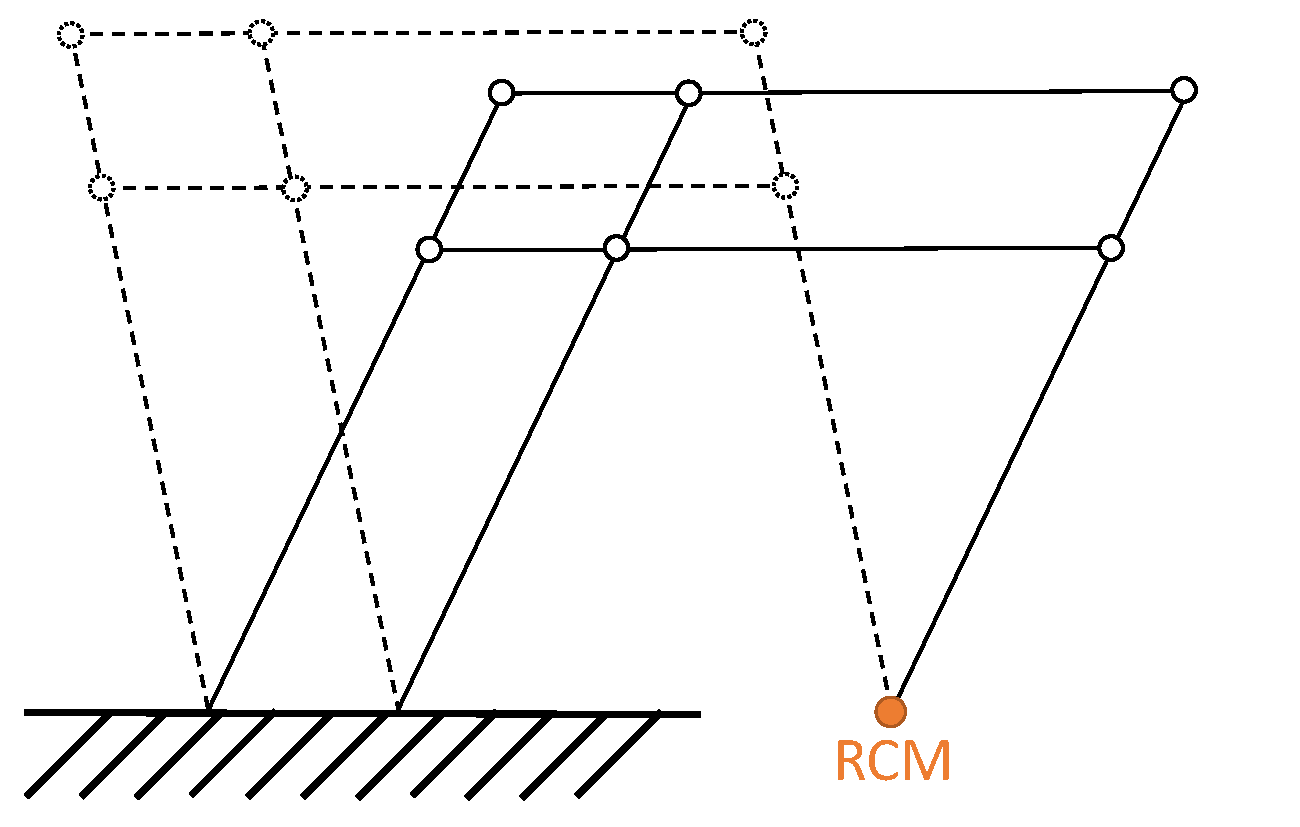
\includegraphics[width=6cm]{mechRCM}
	\caption{A simple, parallelogram based RCM mechanism. The RCM point is mechanically constrained and cannot move relative to the base frame of the robot.}
	\label{mechRCM}
\end{figure}
\begin{figure}[b!]
	\centering
	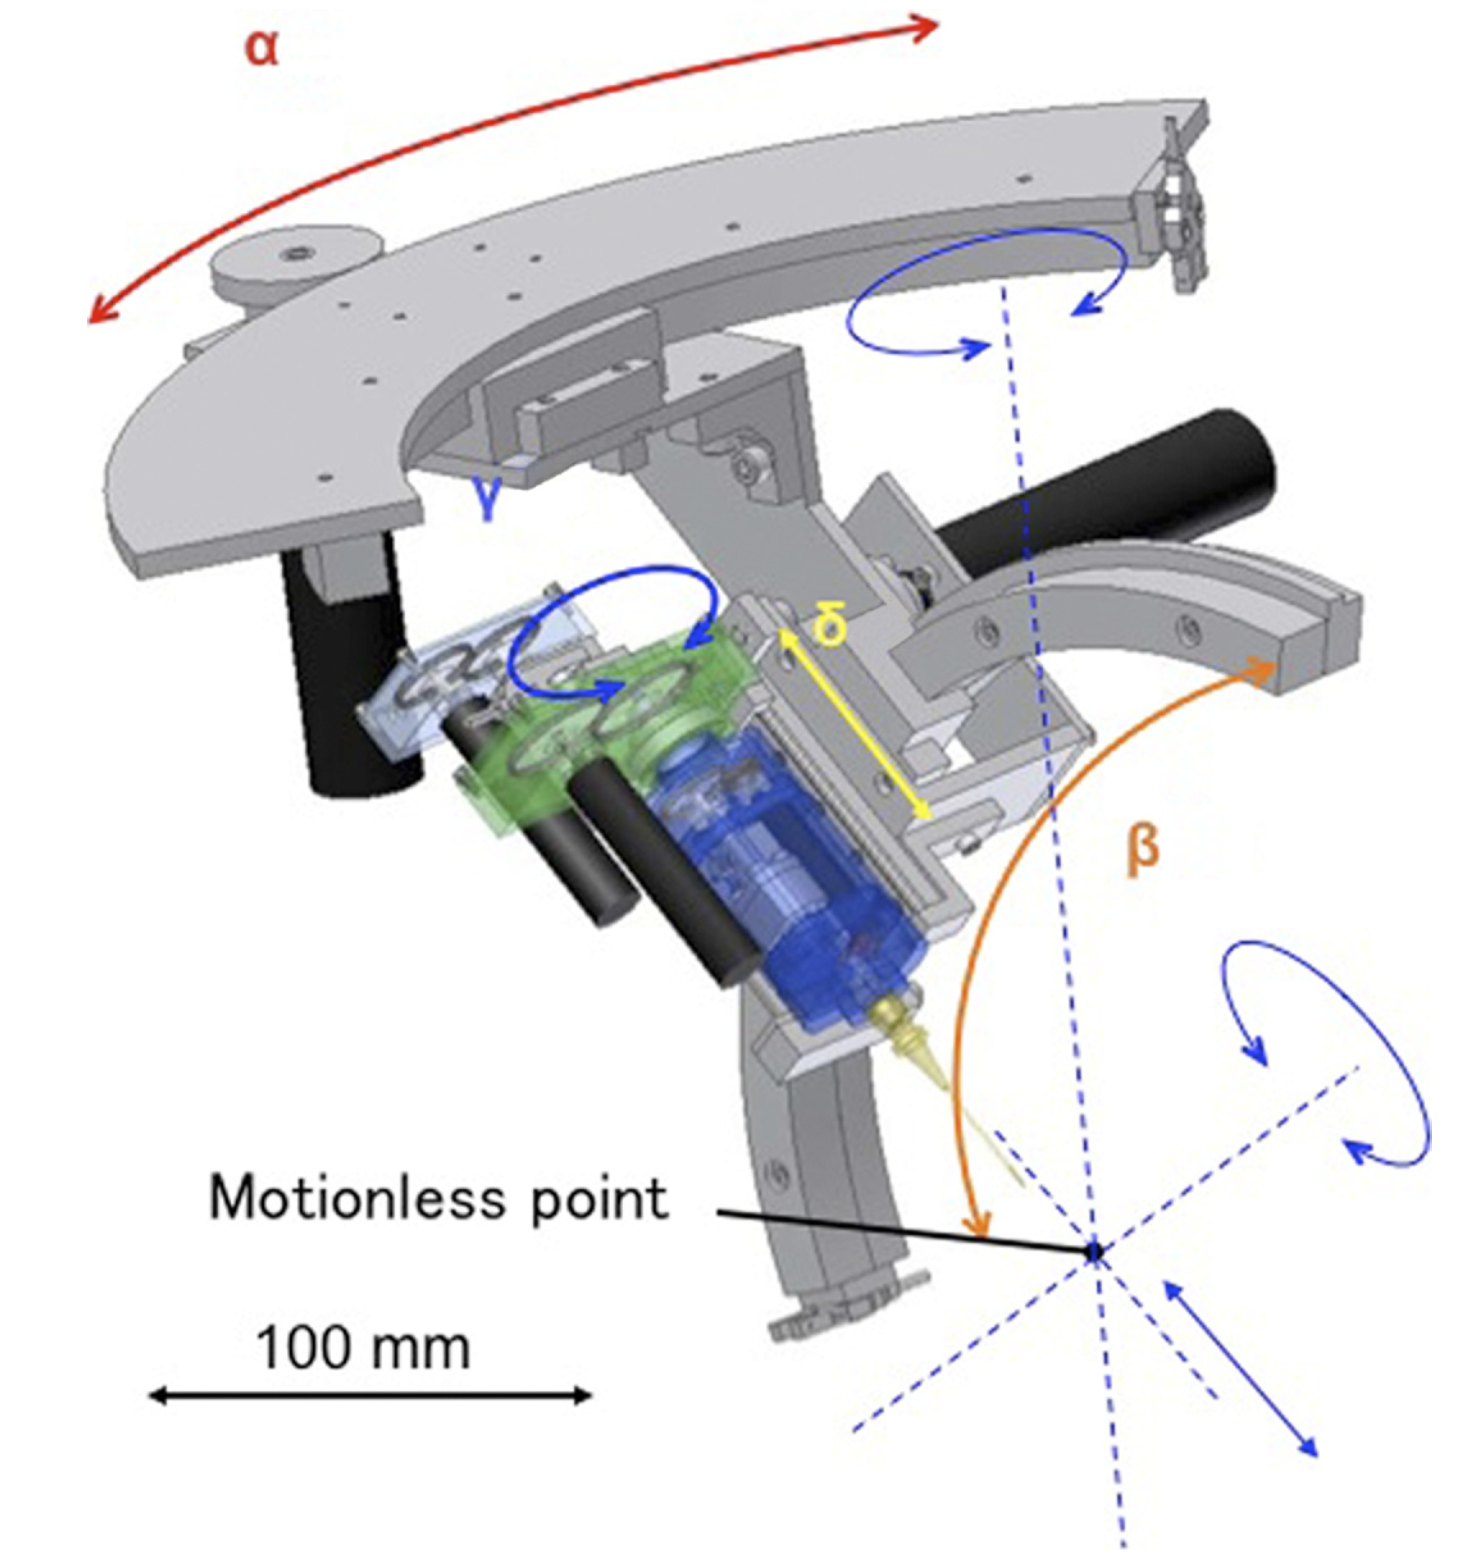
\includegraphics[width=7cm]{Ueta2017_robot}
	\caption{A mechanically constrained robot for ophthalmic surgery developed at the University of Tokyo \cite{Ueta2017}.}
	\label{Ueta2017img}
\end{figure}

Introduction of robots to clinical practice brings several benefits. One major point of interest is to provide smooth, tremor-free position control and force scaling for the tool. Robotic assistance seems especially promising in ophthalmic surgery, which relies on high precision to prevent damage to the delicate tissue of the eye. To minimize damage on the surrounding tissue, movement of the tool laterally to the point of incision must be prevented. While this is a challenging task for a surgeon it is comparably easy for a robot. This concept is referred to as Remote Center of Motion (RCM) and generally divided into two subcategories: \textbf{mechanically constrained} and \textbf{programmable} RCM. 

Examples for a mechanically constrained RCMs are shown in Figures \ref{mechRCM} and \ref{Ueta2017img}. Here, the RCM point is always in the same position relative to the base frame. Mechanically constraining the RCM point is superior in precision and reliability but offers little flexibility in ophthalmic surgery since the position of the robot defines the motionless point and consequently the patient or the whole robot need to be moved until the RCM point coincides with the point of incision.

A programmable RCM, sometimes referred to as a \textit{virtual fixture} \cite{MingLi2004}, is achieved by algorithmically forcing the velocity of an arbitrary point on the manipulator to be zero. This significantly increases the flexibility of the system, but also increases the complexity of the controller required to maintain high precision. Furthermore, a programmable RCM point is in general considered to be less safe than mechanically constrained systems.

The iRAM!S project \cite{nasseri2013introduction} is a joint collaboration of the informatics institute \textit{Robotics and Embedded Systems}, the Graduate School of Information Science in Health (GSISH) and the TUM university hospital Klinikum rechts der Isar. The goal of the project is the development of a novel robotic system for assisting ophthalmic surgeons in complex retinal surgeries, for example for the treatment of diseases such as retinal vein occlusion.

\begin{figure}[t!]
	\centering
	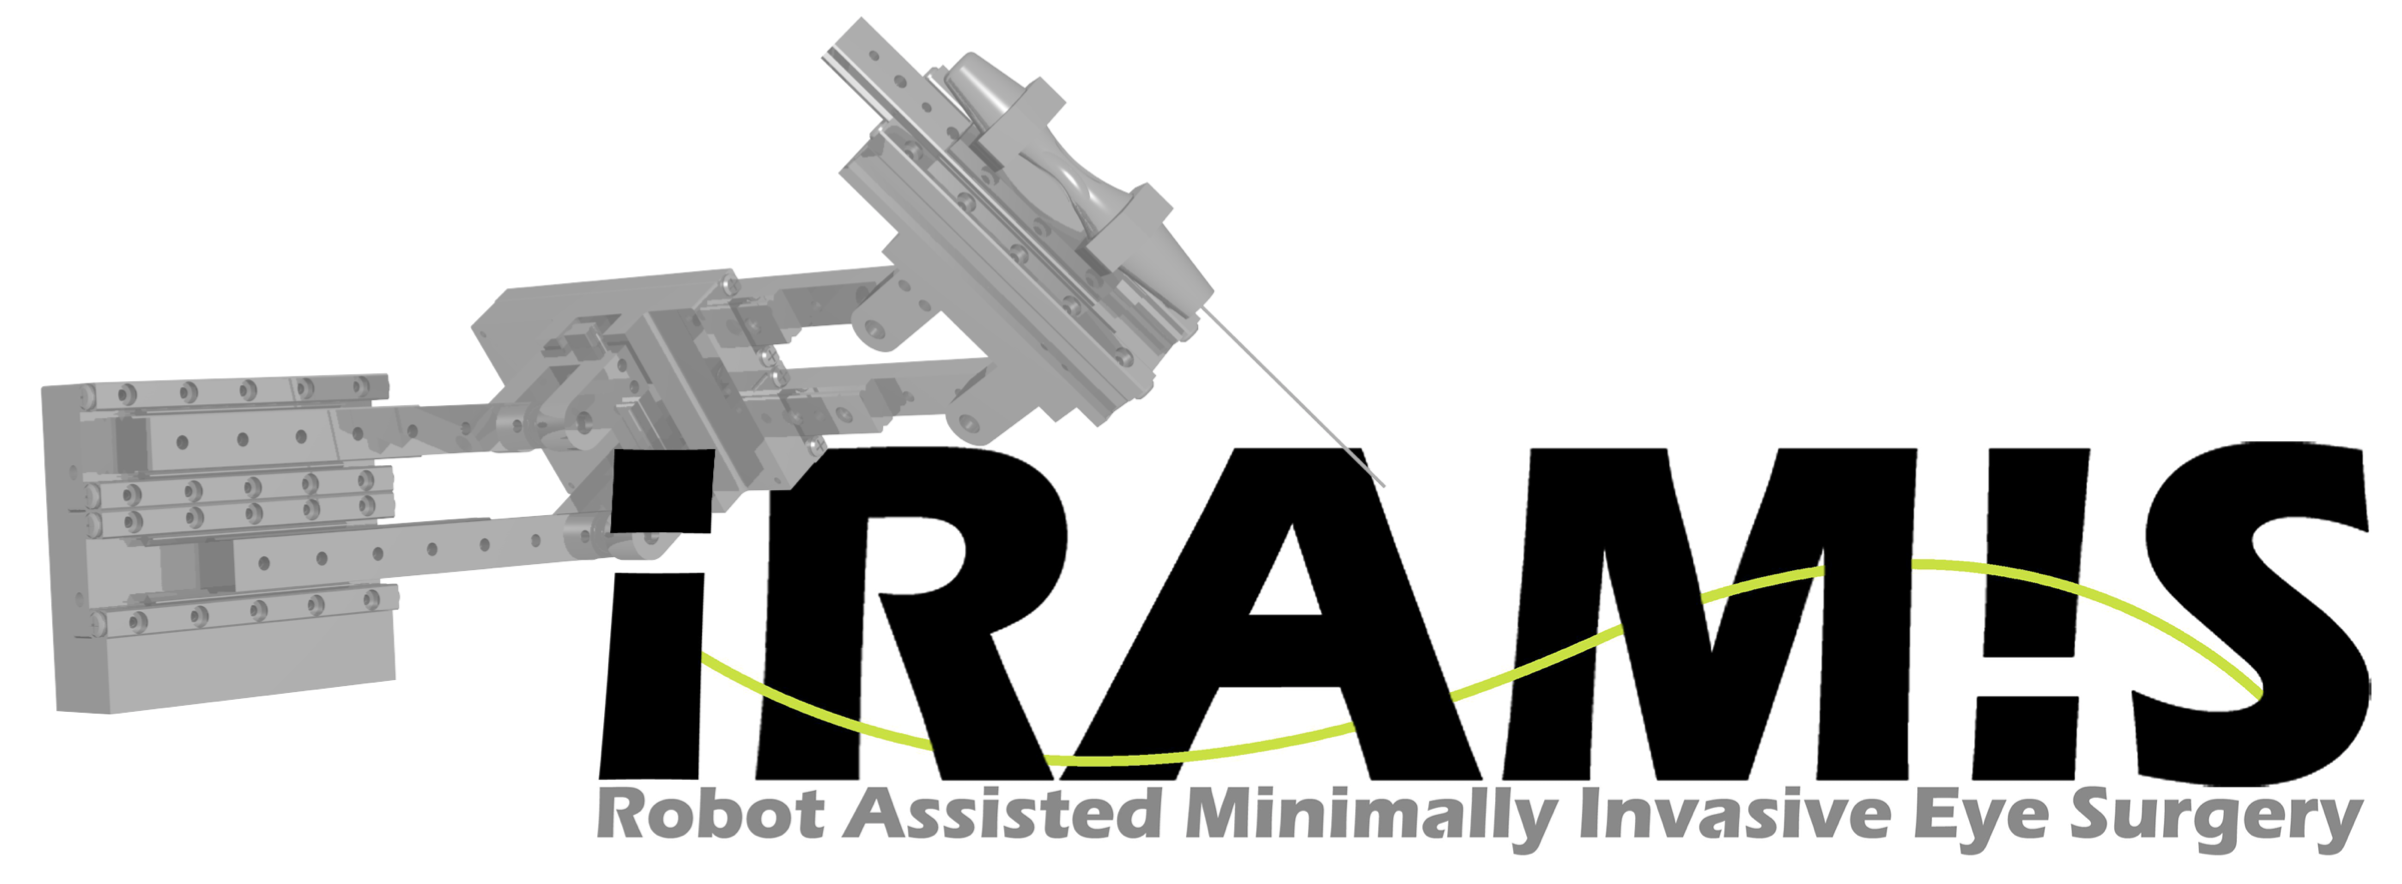
\includegraphics[width=12cm]{iRAM!S}
	\caption{The robotic assistant for ophthalmic surgery developed within the iRAMI!S project \cite{iramis}.}
	\label{iRAM!S}
\end{figure}

\section{Outline}
The second chapter of this thesis describes the mechanical design of the robot and reviews the kinematic relations between joint movements and end effector pose. A step by step description is presented on how to derive the Jacobian from the Denavit-Hartenberg parameters of the robot. 

The Jacobian pseudoinverse approach as a solution for the inverse kinematics problem is introduced, along with the concept of the \textit{augmented Jacobian matrix}, which is used to implement the Remote Center of Motion constraint. Finally, there is a brief introduction to the simulation environment V-REP which will be used to validate the results of the thesis.

In the third chapter, the extended robot task and corresponding Jacobian matrix is defined. A V-REP simulation model is designed from the CAD file and controlled both via a MATLAB remote API and a child script using V-REPs built-in inverse kinematics function. 

In the final Section, the precisions and execution times of both methods are evaluated and compared.